%%%%%%%%%%%%%%%%%%%%%%%%%%%%%%%%%%%%%%%%%
% Template
% LaTeX Template
% Version 1.0 (December 8 2014)
%
% This template has been downloaded from:
% http://www.LaTeXTemplates.com
%
% Original author:
% Brandon Fryslie
% With extensive modifications by:
% Vel (vel@latextemplates.com)
%
% License:
% CC BY-NC-SA 3.0 (http://creativecommons.org/licenses/by-nc-sa/3.0/)
%
% Authors:
% Sabbir Ahmed, Jeffrey Osazuwa, Howard To, Brian Weber
% 
%%%%%%%%%%%%%%%%%%%%%%%%%%%%%%%%%%%%%%%%%

\documentclass[paper=usletter, fontsize=12pt]{article}
%%%%%%%%%%%%%%%%%%%%%%%%%%%%%%%%%%%%%%%%%
% Contract Structural Definitions File Version 1.0 (December 8 2014)
%
% Created by: Vel (vel@latextemplates.com)
% 
% This file has been downloaded from: http://www.LaTeXTemplates.com
%
% License: CC BY-NC-SA 3.0 (http://creativecommons.org/licenses/by-nc-sa/3.0/)
%
%%%%%%%%%%%%%%%%%%%%%%%%%%%%%%%%%%%%%%%%%

\usepackage{geometry} % Required to modify the page layout
\usepackage{multicol}
\usepackage{amsmath}
\usepackage{amssymb}

\usepackage[pdftex]{graphicx}
\usepackage{wrapfig}
\usepackage[font=scriptsize, labelfont=bf]{caption}
\usepackage[utf8]{inputenc} % Required for including letters with accents
\usepackage[T1]{fontenc} % Use 8-bit encoding that has 256 glyphs

\usepackage{avant} % Use the Avantgarde font for headings
\usepackage{courier}
\usepackage{xparse}
\usepackage{xcolor}
\usepackage{listings}  % for code verbatim and console outputs

\setlength{\textwidth}{16cm} % Width of the text on the page
\setlength{\textheight}{23cm} % Height of the text on the page
\setlength{\oddsidemargin}{0cm} % Width of the margin - negative to move text left, positive to move it right
\setlength{\topmargin}{-1.25cm} % Reduce the top margin

\setlength{\parindent}{0mm} % Don't indent paragraphs
\setlength{\parskip}{2.5mm} % Whitespace between paragraphs
\renewcommand{\baselinestretch}{1.5}

\definecolor{green}{rgb}{0.18, 0.55, 0.34}

\graphicspath{ {figures/} }
\captionsetup[table]{skip=10pt}

\lstset{language=C, keywordstyle={\bfseries \color{black}}}

% defines algorithm counter for chapter-level
\newcounter{nalg}[section]

%defines appearance of the algorithm counter
\renewcommand{\thenalg}{\thesection .\arabic{nalg}}

% defines a new caption label as Algorithm x.y
\DeclareCaptionLabelFormat{algocaption}{Algorithm \thenalg}

% defines the algorithm listing environment
\lstnewenvironment{pseudocode}[1][] {
    \refstepcounter{nalg}  % increments algorithm number
    \captionsetup{font=normalsize, labelformat=algocaption, labelsep=colon}
    \lstset{
        breaklines=true,
        mathescape=true,
        numbers=left,
        numberstyle=\scriptsize,
        basicstyle=\footnotesize\ttfamily,
        keywordstyle=\color{black}\bfseries,
        keywords={input, output, return, parallel, function, for, to, in, if,
        else, foreach, while, and, or, new, print},
        xleftmargin=.04\textwidth,
        #1
    }
}{}

\renewcommand{\familydefault}{\sfdefault}  % default font for entire document
 % specifies the document layout and style

%----------------------------------------------------------------------------------------

% document info command
\newcommand{\documentinfo}[5]{
    \begin{centering}
        \parbox{2in}{
        \begin{spacing}{1}
            \begin{flushleft}
                \begin{tabular}{l l}
                    #1 \\
                    #2 \\
                    #3 \\
                \end{tabular}\\
                \rule{\textwidth}{1pt}
            \end{flushleft}
        \end{spacing}
        }
    \end{centering}
}

\begin{document}


    \documentinfo{Sabbir Ahmed}{\textbf{DATE:} \today}{\textbf{CMSC 411} HW 03}
    \vspace{-0.3in}

    \begin{enumerate}

        \item \textbf{Question}
        A digital circuit may be hit by stuck-at faults where one or multiple signals stay always 0 or 1 depending on the fault. Describe the effect that a single stuck-at fault would have for the signals shown below, in the single-cycle datapath shown above and discussed in class. Which instructions, if any, will not work correctly? Explain why.

        Consider each of the following faults separately:

        \begin{enumerate}

            \item RegWrite = 0
            \item ALUSrc = 0
            \item RegDst = 0
            \item Branch = 0
            \item MemWrite = 1

        \end{enumerate}

        \begin{figure}[ht]
            \begin{center}
                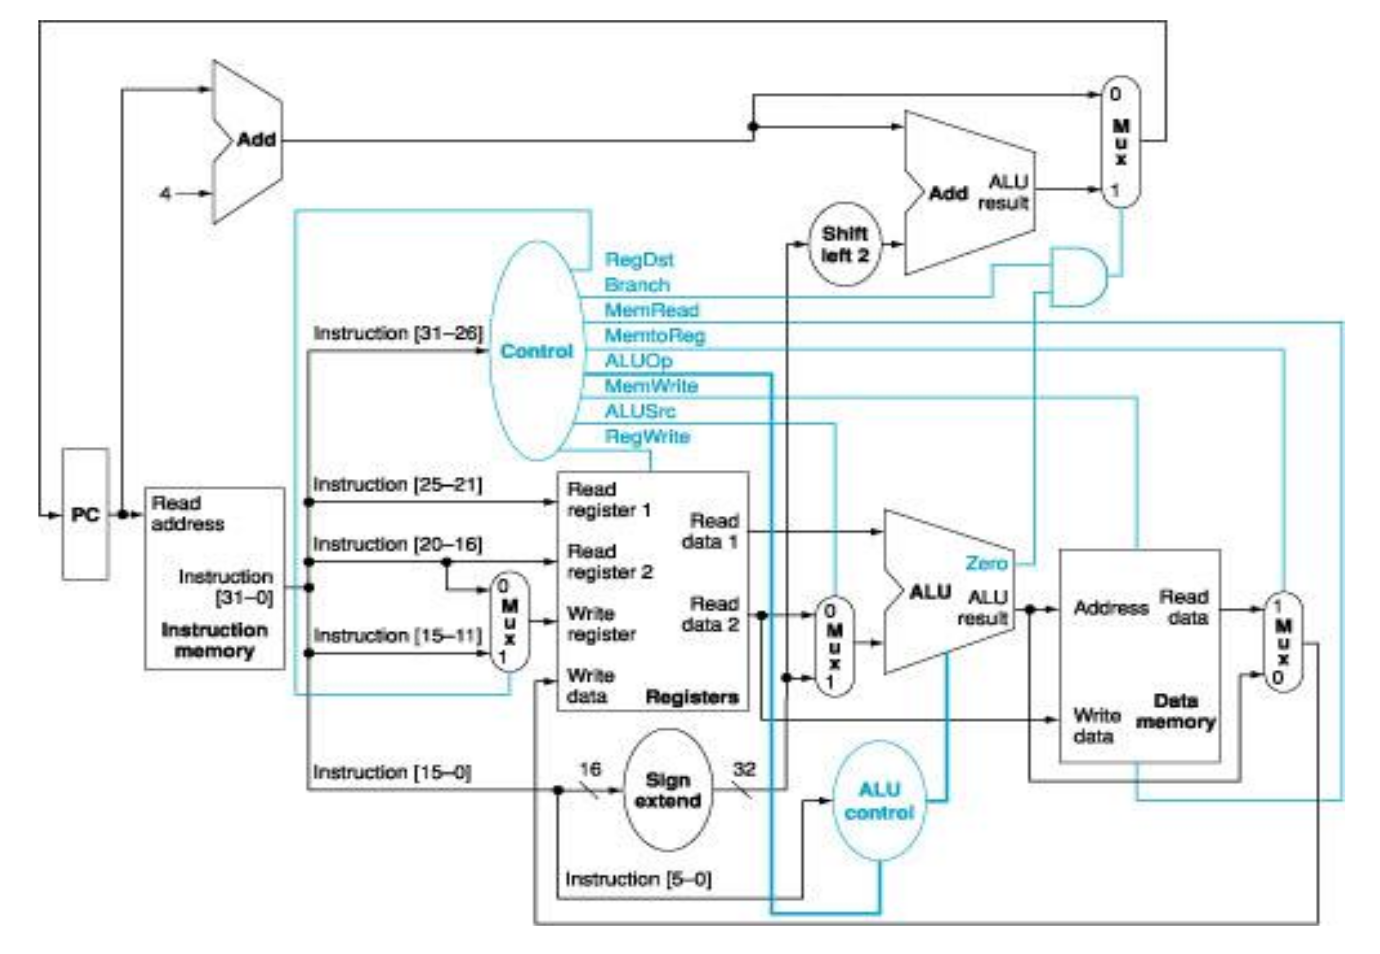
\includegraphics[width=1\textwidth]{circuit.png}
                \caption{Single-Cycle Datapath of the Instructions Described} \label{fig:circuit}
            \end{center}
        \end{figure}

        \textbf{Answer}
        \begin{enumerate}

            \item RegWrite = 0 stuck-at fault would affect the ADD/SUB, ORI and LW instructions. The signal enables the destination register to be written to. The ADD/SUB/ORI instructions perform computations between two registers or a register and an immediate value, and writes the value to the destination register. The LD instruction writes values to destination registers. \\

            \item ALUSrc = 0 stuck-at fault would affect the ORI, LW and SW instructions. These instructions handle immediate values, and would therefore not receive them if the proceeding ALU is only expecting outputs from two registers. \\

            \item RegDst = 0 stuck-at fault would affect the ADD and SUB instructions. The signal enables both the rt and rd registers to contribute their values as required by R-type instructions. \\

            \item Branch = 0 stuck-at fault would only affect the BEQ instruction, since the branch signal would not be enabled to let the program counter know. \\

            \item MemWrite = 1 stuck-at fault would affect the ADD/SUB, ORI, LW and BEQ instructions. The signal enables writing to memory which is not required by any instructions besides SW.

        \end{enumerate}

        \item
        \begin{enumerate}

            \item \textbf{Question}
            We wish to add the instruction “ADDI” (Add immediate) and “LUI” (load upper immediate) to the shown single-cycle simple processor. Add any datapath and control signals and show the value of the control signals while executing the new “ADDI” and “LUI” instruction. \\

            \textbf{Answer}
            The ADDI instruction would not require a separate datapath. The instruction would be identical to ADD, with the only differences being in the following control signals:
            \begin{itemize}
                \item RegDst = 0
                \item ExtOp = 1
                \item ALUSrc = 1
            \end{itemize}
            These are required to enable the immediate value to pass through to the ALU for addition. \\

            The LUI instruction would utilize the same signals as LW, but would require an extra shift register. The shift register would shift-right the immediate value by 16 bits before inputting into the ALU. The updated datapath is as follows: \\

            \begin{figure}[ht]
                \begin{center}
                    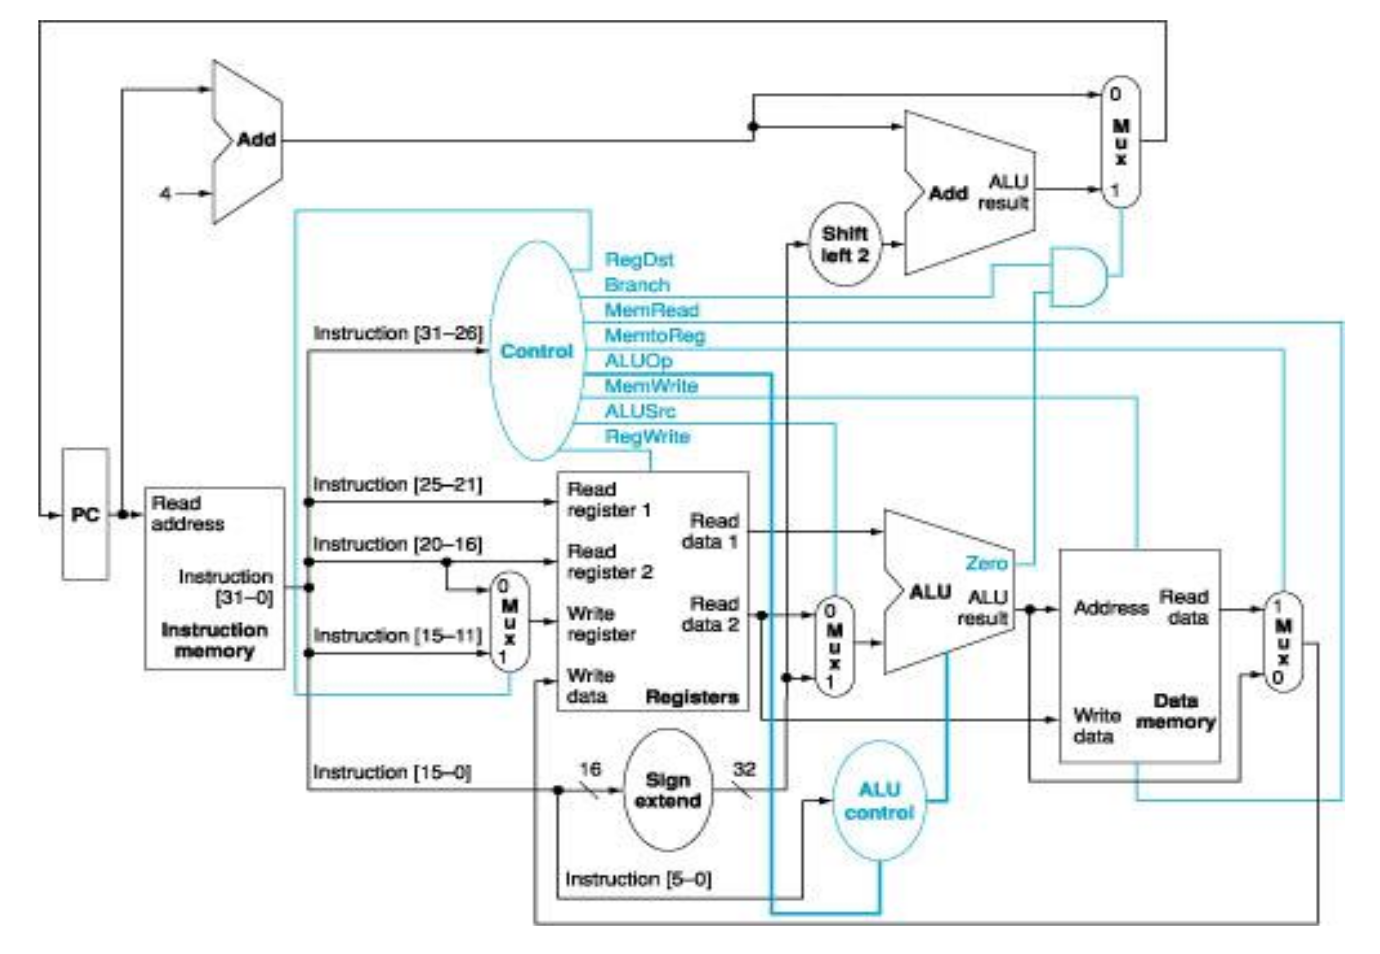
\includegraphics[width=1\textwidth]{circuit.png}
                    \caption{Adding the Datapath for LUI For Question 2A} \label{fig:circuit}
                \end{center}
            \end{figure}
            \newpage

            \item \textbf{Question} This question is similar to part \textbf{A} except that we wish to add a variant of the “LW” (load word) instruction, which increments the index register after loading word from memory. This instruction (“L\_INC”) corresponds to the following two instructions: \\

            LW      \$rs, L(\$rt) \\
            ADDI    \$rt, \$rt, 1 \\

            Again add any datapath and control signals and show the value of the control signals while executing the new instruction. \\
            
            \textbf{Answer} The only difference in the control signal values between LW and ADDI is MemToReg. Therefore, the MemToReg signal could be set to 1, and another 1-bit adder enabled by the L\_INC instruction may be added before the input goes into the multiplexer. The updated datapath is as follows:

            \begin{figure}[ht]
                \begin{center}
                    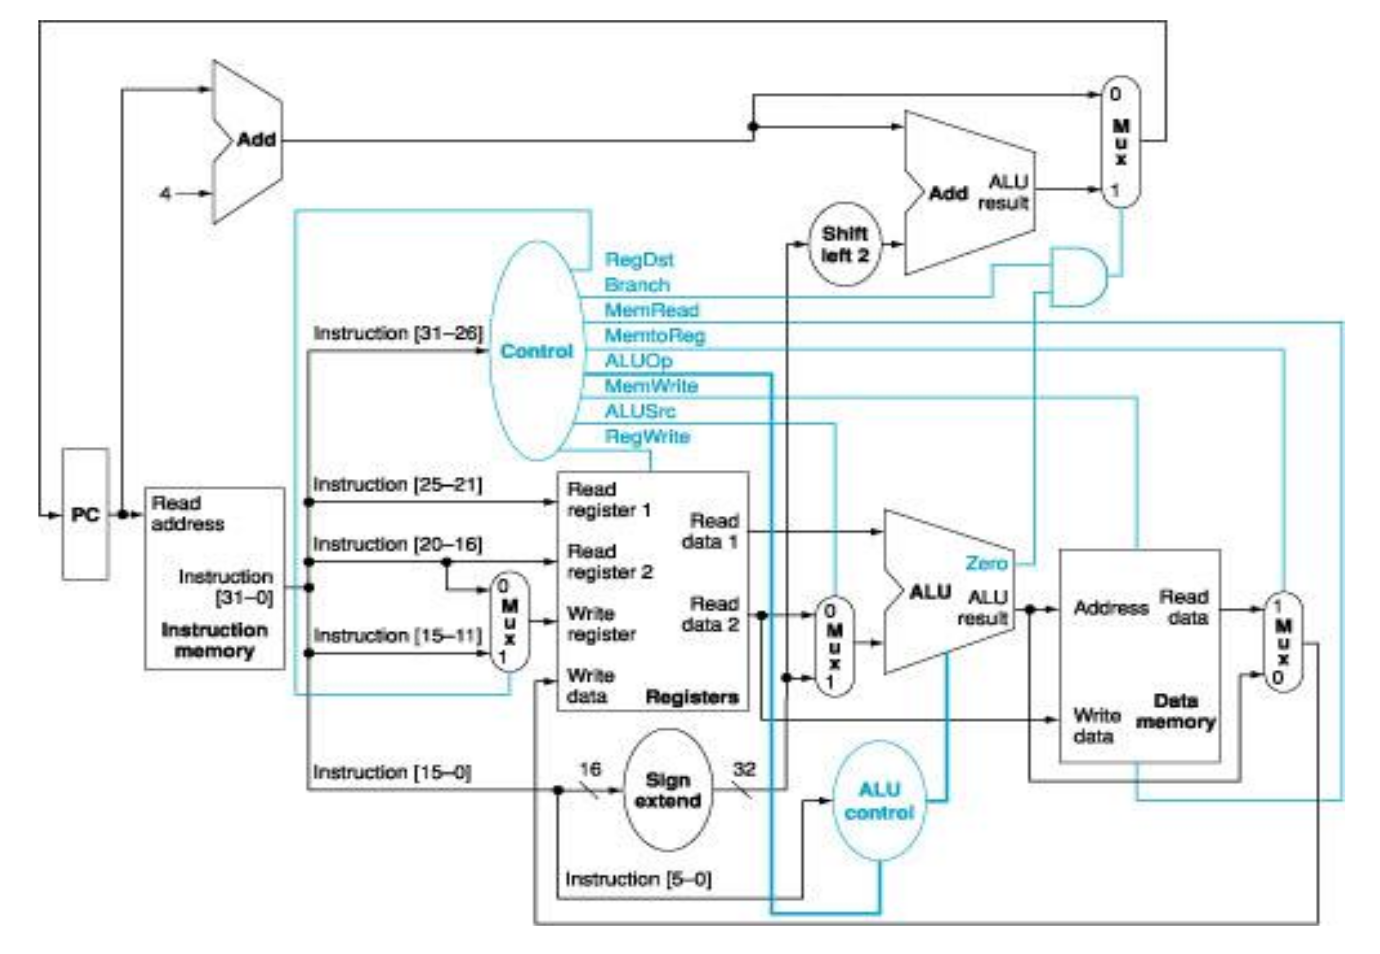
\includegraphics[width=1\textwidth]{circuit.png}
                    \caption{Adding the Datapath for L\_INC For Question 2B} \label{fig:circuit}
                \end{center}
            \end{figure}
            \newpage

        \end{enumerate}

        \item \textbf{Question}
        We wish to add the instruction “JR (jump register)” to the single-cycle datapath shown in question 1. The instruction loads the program counter with the value stored in the specified register. For example, the effect of “JR \$r1” can be summarized as PC $\leftarrow$ [\$r1]. Add any necessary datapaths and control signals and show the value of these control signals when executing all instructions supported by the new datapath.

        \textbf{Answer} The JR instruction would require to load the value from the register, and then increment the program counter with it. This instruction may be implemented by directing the output of the LW instruction directly to the Instruction Fetch Unit. This would increment the program counter similarly to the BEQ instruction; where instead of the PC being equal to PC + 4 + SignExt[imm16]*4 it would equal PC + 4 + [\$r1]*4. The JR control signal would feed into a separate multiplexer proceeding the one following the data memory bank, and would direct the value loaded to the Instruction Fetch Unit. The updated datapath is as follows:

            \begin{figure}[ht]
                \begin{center}
                    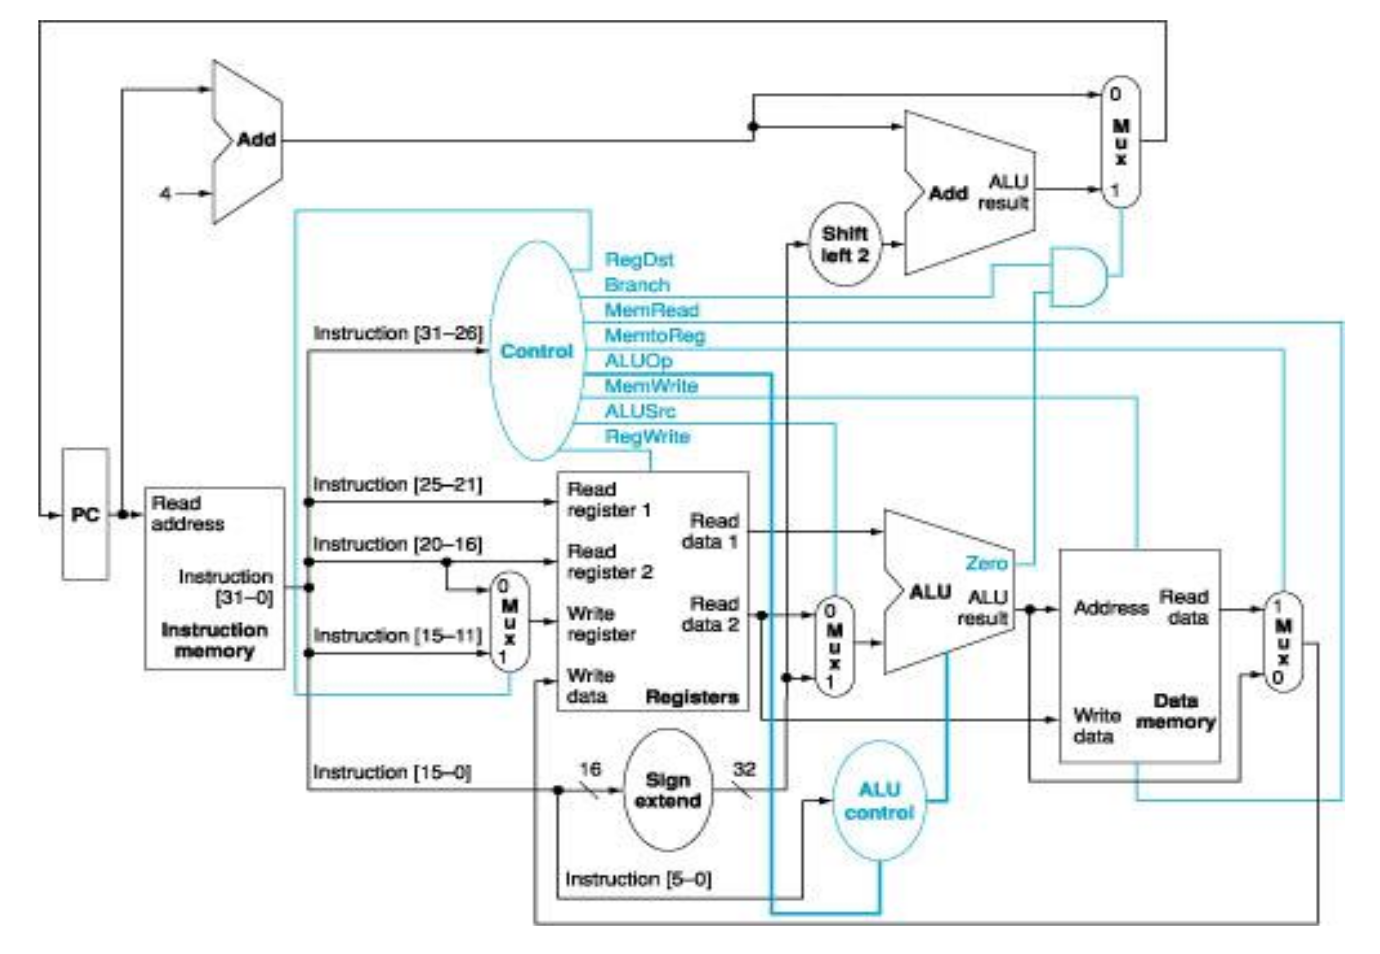
\includegraphics[width=1\textwidth]{circuit.png}
                    \caption{Adding the Datapath for JR For Question 3} \label{fig:circuit}
                \end{center}
            \end{figure}
            \newpage

    \end{enumerate}

\end{document}
